\documentclass[letterpaper]{IEEEtran}

\usepackage{amsmath,amssymb,amsfonts}
\usepackage{graphicx}
\usepackage{textcomp}
\usepackage{xcolor}
\usepackage{booktabs}
\usepackage{multirow}
\usepackage{hyperref}
\usepackage{algorithm}
\usepackage{algorithmic}
\usepackage{subcaption}
\usepackage[capitalize]{cleveref}

% Convenience
\newcommand{\pfail}{P(\text{fail})}
\renewcommand{\rho}{\varrho}
\newcommand{\ie}{\textit{i.e.}}
\newcommand{\eg}{\textit{e.g.}}
\newcommand{\etal}{\textit{et al.}}

% TODO marker
\newcommand{\todo}[1]{\textcolor{red}{\textbf{[TODO: #1]}}}

\begin{document}

\title{Cross-Corruption Safety Monitoring for Vision-Based\\Robot Manipulation via Adversarial Envelope Analysis}

\author{Julian~Quick%
\thanks{Manuscript received XX; revised XX. This work was conducted as an independent research project.}%
\thanks{J.~Quick is an independent researcher. E-mail: quectojoules@gmail.com.}%
\thanks{Digital Object Identifier: to appear.}%
}

\markboth{IEEE Robotics and Automation Letters, Vol.~XX, No.~XX, Month~2026}%
{Quick: Cross-Corruption Safety Monitoring for Vision-Based Robot Manipulation}

\maketitle

% ============================================================================
\begin{abstract}
Vision-language-action (VLA) policies for robot manipulation are brittle under camera occlusion---fingerprints, glare, and rain can degrade success rates from 100\% to near zero.
We present a lightweight safety monitor that predicts manipulation failure probability from a single camera frame, \emph{without requiring the occlusion type to have been seen during training}.
Our approach combines (i)~adversarial worst-case search via CMA-ES to characterize safe operating envelopes across occlusion types and severities, and (ii)~a 33K-parameter CNN head on a frozen ImageNet-pretrained ResNet-18 backbone trained on the resulting labeled episodes.
The key finding is that frozen ImageNet features encode corruption-agnostic visual degradation signals---contrast loss, blur, brightness shifts---that transfer across physically distinct occlusion mechanisms.
A systematic leave-one-out analysis across nine corruption types spanning six physical mechanisms --- lens contact (fingerprint, rain), optical (glare, defocus blur), blur (motion blur), sensor noise, environmental (lens dust), illumination (low-light), and digital (JPEG compression) --- demonstrates that on the six corruption types that cause non-trivial policy failures, the monitor achieves mean Spearman $\rho = 0.79 \pm 0.12$ and mean AUROC $= 0.92 \pm 0.13$ on held-out corruption types it has never encountered.
We additionally characterize how generalization improves with training corruption diversity and identify which corruption categories are easiest and hardest to predict out-of-distribution.
\end{abstract}

\begin{IEEEkeywords}
Safety monitoring, camera occlusion, vision-language-action models, SOTIF, adversarial testing, transfer learning, robot manipulation.
\end{IEEEkeywords}

% ============================================================================
\section{Introduction}
\label{sec:intro}

Vision-language-action (VLA) models such as InternVLA~\cite{internvla}, Octo~\cite{octo}, and RT-2~\cite{rt2} have demonstrated impressive manipulation capabilities, but their reliance on camera observations makes them vulnerable to perceptual degradation.
Recent benchmarking~\cite{liberoplus} reveals that common camera corruptions---fingerprints, glare, rain---can collapse VLA success rates from over 90\% to below 10\%, even at moderate severity levels.

This fragility is a core concern of the Safety of the Intended Functionality (SOTIF, ISO~21448~\cite{iso21448}) standard, which addresses failures arising not from hardware faults but from limitations of perception and decision-making under real-world conditions.
Camera occlusion is a canonical SOTIF triggering condition for vision-based systems: it is ubiquitous in deployment (warehouse dust, outdoor rain, operator fingerprints on lenses) yet difficult to anticipate exhaustively.

A practical safety monitor must therefore satisfy two requirements: (1)~it must detect when occlusion severity is likely to cause policy failure, and (2)~it must generalize to occlusion types \emph{not encountered during training}, since enumerating all possible degradation modes is infeasible.

We address both requirements with a two-stage approach.
First, we use adversarial optimization via CMA-ES~\cite{cmaes} to systematically find worst-case occlusion parameters at each severity (budget) level, producing a \emph{safe operating envelope} that maps occlusion coverage to certified success rates (\cref{sec:envelope}).
Second, we train a lightweight CNN safety monitor on the resulting labeled episodes and evaluate its ability to generalize to held-out corruption types (\cref{sec:safety_predictor}).

Our key finding is that a frozen ImageNet-pretrained ResNet-18 backbone, paired with a small trainable head (33K parameters), learns corruption-agnostic failure signals that transfer across physically distinct occlusion mechanisms.
Trained on fingerprint and glare corruptions, the monitor achieves strong rank correlation with failure probability under rain occlusion it has never seen.

\noindent\textbf{Contributions:}
\begin{enumerate}
    \item A systematic leave-one-out evaluation across nine corruption types spanning six physical mechanisms, demonstrating corruption-agnostic failure detection.
    \item A lightweight cross-corruption safety monitor (33K trainable parameters) that generalizes to unseen occlusion types via frozen pretrained features.
    \item A predictor of OOD detection quality from feature-delta similarity to the training set, enabling deployment-time forecasting of monitor reliability on novel corruption types without ground-truth failure labels.
    \item An adversarial envelope analysis framework using CMA-ES to characterize worst-case policy performance under parametric occlusion.
\end{enumerate}

% ============================================================================
\section{Related Work}
\label{sec:related}

\subsection{Robustness of Vision-Based Manipulation Policies}

Recent work has exposed the fragility of learned manipulation policies under visual corruptions.
LIBERO-Plus~\cite{liberoplus} systematically benchmarks VLA robustness, finding dramatic performance drops under ImageNet-C-style corruptions.
RobustVLA~\cite{robustvla} proposes robustness-aware reinforcement learning post-training to harden policies.
FPC-VLA~\cite{fpcvla} combines failure prediction with corrective actions.
CRT~\cite{crt} restores corrupted visual inputs before feeding them to VLA policies.
These approaches either make the policy more robust or restore corrupted inputs; our work is complementary---we build an external safety monitor that detects when the policy is likely to fail, regardless of whether the policy or input has been hardened.

\subsection{Runtime Safety Monitoring}

Sentinel~\cite{sentinel} monitors generative manipulation policies at runtime by detecting behavioral anomalies at the policy output level.
Ma~\etal~\cite{ma2024} predict failure from camera faults using multimodal features with 4000 real-world samples.
FORTRESS~\cite{fortress} addresses real-time out-of-distribution failure prevention.
Our approach differs in monitoring at the \emph{perceptual input level} and demonstrating zero-shot generalization to unseen corruption types---a property not evaluated in prior work.

\subsection{Adversarial Testing for Safety}

Adversarial testing has been used to find failure modes in autonomous driving~\cite{adv_driving} and manipulation~\cite{adv_manip}.
CMA-ES is well-suited for this setting as it is derivative-free, handles moderate-dimensional parameter spaces efficiently, and naturally parallelizes across population members.
We extend adversarial testing to produce certified safe operating envelopes parameterized by occlusion severity.

\subsection{SOTIF and Safety Standards}

ISO~21448~\cite{iso21448} defines a framework for analyzing safety of the intended functionality, distinguishing known/unknown safe and unsafe scenarios.
Our envelope analysis maps directly to SOTIF's scenario classification: adversarially tested conditions become ``known unsafe,'' while cross-corruption generalization moves previously ``unknown unsafe'' scenarios toward ``known'' status.
We develop the mapping formally in \cref{sec:sotif}.

% ============================================================================
\section{Problem Formulation}
\label{sec:problem}

Consider a vision-based manipulation policy $\pi$ that maps camera observations $o_t \in \mathbb{R}^{H \times W \times 3}$ to actions $a_t$.
An occlusion model $\mathcal{O}_\theta: \mathbb{R}^{H \times W \times 3} \to \mathbb{R}^{H \times W \times 3}$ parameterized by $\theta \in \Theta$ degrades the observation at each timestep: $\tilde{o}_t = \mathcal{O}_\theta(o_t, t)$.
A budget function $b(\theta) \in [0, 1]$ quantifies occlusion severity: for spatially-localized corruptions it measures the fraction of pixels significantly affected by the occlusion, while for global corruptions it acts as a normalized cap on the corruption intensity (\cref{sec:budget_constraint}).

\noindent\textbf{Safe Operating Envelope.}
For a given occlusion type $\mathcal{O}$ and budget level $\beta$, we seek the worst-case success rate:
\begin{equation}
    \text{SR}^*(\mathcal{O}, \beta) = \min_{\theta : b(\theta) \leq \beta} \; \mathbb{E}\left[\text{success}(\pi, \mathcal{O}_\theta)\right]
\label{eq:envelope}
\end{equation}
The safe operating envelope is the set of $(\mathcal{O}, \beta)$ pairs where $\text{SR}^*(\mathcal{O}, \beta) \geq \tau_{\text{safe}}$.

\noindent\textbf{Safety Monitor.}
We train a monitor $f_\phi: \mathbb{R}^{H \times W \times 3} \to [0, 1]$ that maps a single (potentially occluded) frame to a predicted failure probability $\hat{p} = f_\phi(\tilde{o}_t)$.
The monitor is trained on corruption types $\mathcal{O}_{\text{train}}$ and evaluated on held-out types $\mathcal{O}_{\text{test}}$ to assess cross-corruption generalization.

% ============================================================================
\section{Parametric Occlusion Models}
\label{sec:occlusion}

We organize visual corruptions by physical mechanism following the taxonomy of Hendrycks \& Dietterich~\cite{hendrycks2019}, adapted for fixed-mount robot cameras.
Our set spans six categories to support systematic cross-corruption generalization analysis.
All corruptions are applied as image-space post-processing on rendered camera frames and are parameterized with a budget level $\beta \in [0, 1]$ controlling severity.

\cref{tab:corruptions} summarizes the nine corruption types used in our experiments.

\begin{table}[t]
\centering
\caption{Corruption taxonomy organized by physical mechanism.}
\label{tab:corruptions}
\footnotesize
\begin{tabular}{llrl}
\toprule
\textbf{Category} & \textbf{Corruption} & \textbf{Params} & \textbf{Source} \\
\midrule
Lens contact  & Fingerprint smudge & 24 & Gu~\etal~\cite{gu2009} \\
Lens contact  & Rain drops         &  5 & \cite{camera_occlusion} \\
Optical       & Glare / lens flare &  6 & Physically-inspired \\
Optical       & Defocus blur       &  1 & ImageNet-C~\cite{hendrycks2019} \\
Blur          & Motion blur        &  2 & ImageNet-C~\cite{hendrycks2019} \\
Sensor        & Gaussian noise     &  2 & ImageNet-C~\cite{hendrycks2019} \\
Environmental & Dust on lens       &  4 & Physically-inspired \\
Illumination  & Low-light          &  2 & LIBERO-Plus~\cite{liberoplus} \\
Digital       & JPEG compression   &  1 & ImageNet-C~\cite{hendrycks2019} \\
\bottomrule
\end{tabular}
\end{table}

\subsection{Physics-Based Models}

\noindent\textbf{Fingerprint smudge.}
Based on the thin-film optics model of Gu~\etal~\cite{gu2009}, we simulate oil-film residue from finger contact.
Each fingerprint is parameterized by center, angle, scale, ridge frequency, amplitude, opacity, and smear angle (8 parameters per print).
The rendering pipeline generates a whorl-pattern ridge mask, applies defocus blur, and composites via attenuation and veiling glare.

\noindent\textbf{Glare / lens flare.}
We model lens flare as diffraction spikes, haze, chromatic aberration, and lens ghosts.
Compositing uses screen blending: $I_{\text{out}} = 1 - (1 - I_{\text{base}})(1 - I_{\text{flare}})$.

\noindent\textbf{Rain drops.}
Refraction-based raindrop model~\cite{camera_occlusion} parameterized by drop density, radius range, magnification, and blur.

\subsection{Standard Corruption Models}

Following ImageNet-C~\cite{hendrycks2019} and LIBERO-Plus~\cite{liberoplus}, we include:
\textbf{Gaussian noise} (additive sensor read noise),
\textbf{JPEG compression} (block artifacts at controllable quality),
\textbf{motion blur} (directional kernel with variable angle and size),
\textbf{defocus blur} (Gaussian blur with variable sigma),
\textbf{lens dust} (randomly sampled ellipsoidal opaque patches on the lens), and
\textbf{low-light} (gamma darkening with amplified sensor read noise, simulating reduced photon count).

\subsection{Budget Constraint}
\label{sec:budget_constraint}

All models enforce a budget level $\beta$ controlling corruption severity.
For spatially-localized models (fingerprint, glare), budget is the fraction of pixels above a dirty threshold, enforced via a binary-search projection step.
For global models (rain, noise, JPEG, motion and defocus blur, low-light, lens dust), budget acts as a multiplicative cap on the corruption intensity parameter.
This enables fair comparison across corruption types at matched severity levels.

\begin{figure}[t]
    \centering
    
\includegraphics[width=\columnwidth]{figures/corruption_grid.png}
    \caption{Sample frames from all nine corruption types at matched budget $\beta = 0.5$. The taxonomy spans lens contact, optical, blur, sensor, environmental, illumination, and digital mechanisms, chosen to systematically probe cross-corruption generalization.}
    \label{fig:corruption_grid}
\end{figure}

% ============================================================================
\section{Adversarial Envelope Analysis}
\label{sec:envelope}

\subsection{CMA-ES Optimization}

We use the Covariance Matrix Adaptation Evolution Strategy (CMA-ES)~\cite{cmaes} to solve \cref{eq:envelope} for each occlusion type and budget level.
CMA-ES is well-suited because: (i)~occlusion application is non-differentiable, (ii)~the parameter space is moderate-dimensional (6--24 dimensions), and (iii)~population-based evaluation naturally parallelizes across simulation instances.

At each generation, CMA-ES proposes a population of candidate occlusion parameters $\{\theta_1, \ldots, \theta_\lambda\}$.
Each candidate is evaluated by running $N$ episodes with the occluded policy and computing the success rate.
The fitness (negative success rate) is reported back to CMA-ES, which updates its search distribution.
After convergence, the best candidate undergoes a final evaluation with $N_{\text{final}} = 25$ episodes.

\subsection{Budget Projection}

To ensure fair comparison across budget levels, all occlusion models implement a budget projection step.
Given a target budget $\beta$, we perform binary search over a global scale factor that modulates occlusion intensity until the pixel coverage constraint $b(\theta) \leq \beta$ is satisfied.
This decouples the spatial structure of the occlusion (optimized by CMA-ES) from its intensity (set by the budget).

\subsection{Envelope Classification}

We classify each $(\mathcal{O}, \beta)$ condition into zones:
\begin{itemize}
    \item \textbf{Safe}: $\text{SR}^*(\mathcal{O}, \beta) \geq 0.95$
    \item \textbf{Marginal}: $0.70 \leq \text{SR}^*(\mathcal{O}, \beta) < 0.95$
    \item \textbf{Unsafe}: $\text{SR}^*(\mathcal{O}, \beta) < 0.70$
\end{itemize}
The \emph{maximum safe budget} is the largest $\beta$ for which the condition remains safe.
The \emph{breakdown budget} is the smallest $\beta$ at which the condition becomes unsafe.

Envelope results are reported in \cref{sec:envelope_results}.

% ============================================================================
\section{Cross-Corruption Safety Monitor}
\label{sec:safety_predictor}

\subsection{Architecture}

Our safety monitor uses a ResNet-18~\cite{resnet} backbone pretrained on ImageNet~\cite{imagenet}, with all backbone parameters frozen.
A lightweight classification head maps the 512-dimensional feature vector to a scalar failure logit:
\begin{equation}
    f_\phi(o) = \sigma\!\left(W_2 \cdot \text{ReLU}(W_1 \cdot g(o) + b_1) + b_2\right)
\end{equation}
where $g(\cdot)$ denotes the frozen ResNet-18 feature extractor, $W_1 \in \mathbb{R}^{64 \times 512}$, $W_2 \in \mathbb{R}^{1 \times 64}$, and $\sigma$ is the sigmoid function.
Dropout ($p = 0.3$) is applied after the ReLU.
The head contains approximately 33K trainable parameters.

\subsection{Training}

\noindent\textbf{Data collection.}
For each training corruption type (fingerprint, glare) and budget level $\beta \in \{0.1, 0.3, 0.5, 0.7, 0.9\}$, we collect episodes with both random and adversarially optimized occlusion parameters.
Each episode yields sampled frames labeled with the episode outcome (success/failure).

\noindent\textbf{Loss function.}
We use binary cross-entropy with logits and class weighting to handle imbalanced data:
\begin{equation}
    \mathcal{L} = -\frac{1}{N}\sum_{i=1}^{N} \left[w_+ y_i \log \hat{p}_i + (1 - y_i) \log (1 - \hat{p}_i)\right]
\end{equation}
where $w_+ = n_{\text{success}} / n_{\text{failure}}$ upweights the minority failure class.

\noindent\textbf{Episode-level splitting.}
To prevent data leakage from temporally correlated frames within the same episode, we split at the episode level: all frames from a given episode appear exclusively in either the training or validation set ($80/20$ split).

\noindent\textbf{Optimization.}
Adam optimizer with learning rate $10^{-3}$, batch size 32, for 50 epochs with ReduceLROnPlateau scheduling.

\subsection{Leave-One-Out Cross-Corruption Protocol}
\label{sec:loo}

To systematically evaluate cross-corruption generalization, we employ a leave-one-out (LOO) protocol over all nine corruption types.
In each fold $k$, one corruption type $\mathcal{O}_k$ is held out.
The safety monitor is trained on episodes collected from the remaining eight types and evaluated on the held-out type.

For each held-out type we sweep five budget levels $\beta \in \{0.1, 0.3, 0.5, 0.7, 0.9\}$, running $N$ evaluation episodes per level, and compute:
\begin{itemize}
    \item The Spearman rank correlation $\rho$ between the empirical failure rate (one minus the measured episode success rate) and the mean predicted $\hat{p}_{\text{fail}}$, taken across the five budget levels (severity ranking quality). Budget indexes the five conditions being correlated; it is not itself one of the correlated variables.
    \item The episode-level AUROC for binary failure prediction (discriminative power).
    \item The Expected Calibration Error (ECE) from reliability diagrams.
\end{itemize}
Bootstrapped 95\% confidence intervals (1000 resamples) are reported for all metrics.
Note that the per-fold $\rho$ is computed over only $n=5$ condition points (the five budget levels), whereas AUROC is computed over all $n=50$ episodes in the fold; AUROC is therefore the statistically stronger of the two metrics.

\noindent\textbf{Corruption diversity curve.}
We additionally vary the training set size $|\mathcal{O}_{\text{train}}| \in \{2, 4, 6, 8\}$ by randomly sampling subsets and evaluating on the remaining types.
This reveals how many corruption types are needed for effective generalization.

% ============================================================================
\section{Experiments}
\label{sec:experiments}

\subsection{Experimental Setup}

\noindent\textbf{Simulation.}
We use SimplerEnv~\cite{simplerenv} built on SAPIEN/ManiSkill2 for policy evaluation.
Corruptions are applied as post-processing on rendered camera frames at each simulation step.
Object positions are randomized at each episode reset.

\noindent\textbf{Policy.}
InternVLA-M1~\cite{internvla}, a vision-language-action model, serves as the manipulation policy.
On the \texttt{google\_robot\_pick\_coke\_can} task, it achieves 100\% success rate (50/50 episodes) under clean conditions.

\noindent\textbf{Data collection.}
For each of the nine corruption types (\cref{tab:corruptions}) at budget levels $\beta \in \{0.1, 0.3, 0.5, 0.7, 0.9\}$, we collect 10 episodes with random occlusion parameters, yielding ${\sim}450$ episodes total.
Each episode contributes sampled frames labeled with the episode outcome (success/failure).
This shared dataset is partitioned differently for each LOO fold, making the CNN training cost negligible (33K parameters, ${\sim}$2 minutes per fold).

\subsection{Motivating Experiment}

In preliminary experiments, we trained the safety monitor on only fingerprint and glare corruptions and evaluated on held-out rain.
A from-scratch CNN achieved $\rho = -0.62$ (anti-correlated), while the frozen ResNet-18 backbone achieved $\rho = 0.90$ ($p = 0.037$).
This surprising result --- a 152-percentage-point improvement from pretrained features alone --- motivated the systematic LOO analysis that follows.

\subsection{Leave-One-Out Results}

\begin{table}[t]
\centering
\caption{Leave-one-out cross-corruption generalization. Each row holds out one corruption type; the monitor is trained on the other eight. Higher $\rho$ and AUROC indicate better OOD generalization. Three corruption types (glare, Gaussian noise, JPEG) did not induce measurable policy failures at the tested budgets on this task and so yield no variance for severity ranking---these are marked ``n/a'' and excluded from the mean.}
\label{tab:loo}
\footnotesize
\setlength{\tabcolsep}{4pt}
\begin{tabular}{@{}llccc@{}}
\toprule
\textbf{Category} & \textbf{Held-out} & \textbf{$\rho$} & \textbf{95\% CI} & \textbf{AUROC} \\
\midrule
Lens contact  & Rain          & 1.000 & $[1.00, 1.00]$ & 0.981 \\
Optical       & Defocus blur  & 0.894 & $[0.73, 1.00]$ & 0.973 \\
Environmental & Lens dust     & 0.783 & $[0.11, 1.00]$ & 0.943 \\
Blur          & Motion blur   & 0.707 & $[0.71, 1.00]$ & 1.000 \\
Illumination  & Low-light     & 0.707 & $[0.71, 1.00]$ & 1.000 \\
Lens contact  & Fingerprint   & 0.667 & $[-0.91, 1.00]$ & 0.636 \\
\midrule
Optical       & Glare         & n/a   & ---            & n/a   \\
Sensor        & Gauss.\ noise & n/a   & ---            & n/a   \\
Digital       & JPEG          & n/a   & ---            & n/a   \\
\midrule
\multicolumn{2}{l}{\textbf{Mean $\pm$ std} (6 failing types)} & $0.79 \pm 0.12$ & --- & $0.92 \pm 0.13$ \\
\bottomrule
\end{tabular}
\end{table}

\begin{figure}[t]
    \centering
    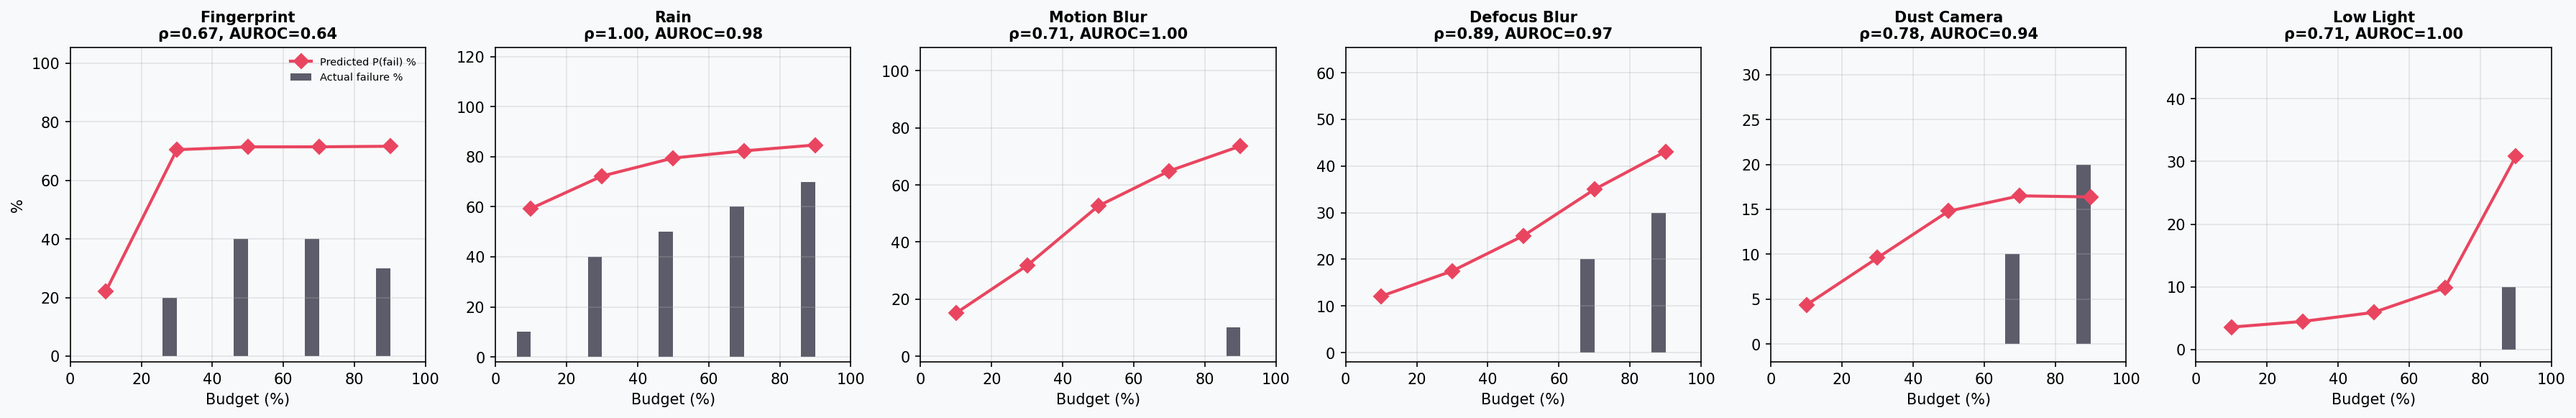
\includegraphics[width=\columnwidth]{figures/loo_per_fold.png}
    \caption{Per-fold leave-one-out results. Each panel shows mean predicted failure probability (bars) versus budget level for the held-out corruption type; the monitor was trained only on the other eight types. Monotone bars indicate successful severity ranking under a previously unseen corruption.}
    \label{fig:loo_per_fold}
\end{figure}

\cref{tab:loo} reports the LOO results.
Of the nine corruption types, three (glare, Gaussian noise, JPEG) do not cause policy failures at any budget in our set and therefore yield degenerate (constant) rankings; we report the six remaining types, where failures are observed and severity ranking is meaningful.
Across these six, the monitor achieves mean Spearman $\rho = 0.79 \pm 0.12$ and mean AUROC $= 0.92 \pm 0.13$ despite never having seen the held-out corruption during training.

The easiest generalization target is \textbf{rain} ($\rho = 1.00$, AUROC $= 0.98$): rain shares the lens-contact family with the training corruption fingerprint, and both produce localized contrast attenuation and low-frequency smearing that the frozen backbone encodes similarly.
\textbf{Defocus blur} and \textbf{motion blur} likewise generalize well (AUROC $\geq 0.97$): both reduce high-frequency texture, a signal the ImageNet features capture reliably.
\textbf{Fingerprint} is the hardest target ($\rho = 0.67$, AUROC $= 0.64$) --- it is structurally distinctive (spatially localized whorl ridges, strong anisotropy) and has no close analogue among the remaining eight training corruptions when it is held out.
This asymmetry --- rain generalizes from fingerprint but not vice versa --- suggests that the monitor relies on \emph{information-content} features that are reduced by any contrast-loss corruption, and that idiosyncratic structural signatures (localized ridges) require in-distribution exposure.

\subsection{Calibration}
\label{sec:calibration}

We complement the ranking metrics ($\rho$, AUROC) with Expected Calibration Error (ECE), measured by binning episode-level $\hat{p}_{\text{fail}}$ into 10 equal-width bins and comparing each bin's mean prediction to the empirical failure rate within it.
\cref{fig:reliability} shows the pooled reliability diagram across all six failing held-out corruption types ($n = 300$ episodes); per-fold ECE values are reported in \cref{tab:ece}.

\begin{figure}[t]
    \centering
    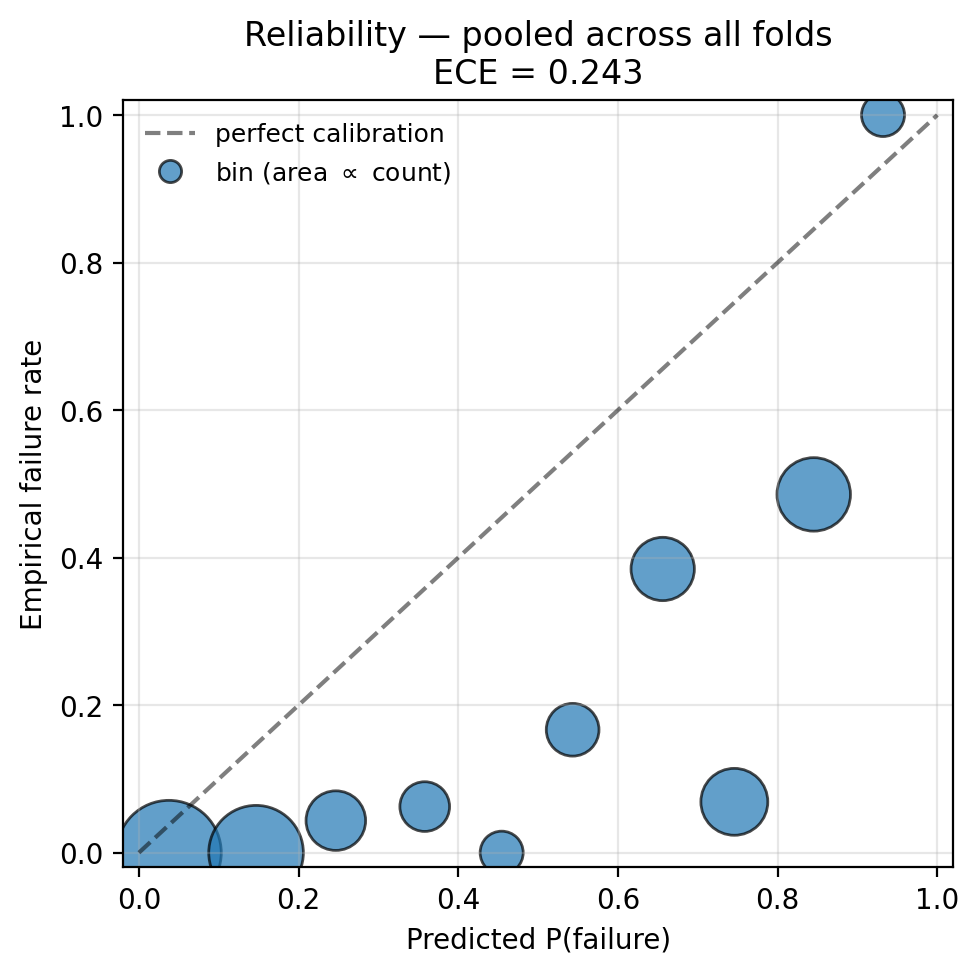
\includegraphics[width=0.85\columnwidth]{figures/reliability_pooled.png}
    \caption{Pooled reliability diagram across the six LOO held-out corruption types that produced measurable failures. Bin marker size is proportional to the number of episodes in the bin. The monitor is well-ordered (positively sloped) but systematically over-confident at high predicted-failure values --- pooled ECE = 0.243.}
    \label{fig:reliability}
\end{figure}

\begin{table}[t]
\centering
\caption{Per-fold Expected Calibration Error and Maximum Calibration Error.}
\label{tab:ece}
\footnotesize
\setlength{\tabcolsep}{4pt}
\begin{tabular}{@{}lcc@{}}
\toprule
\textbf{Held-out} & \textbf{ECE} & \textbf{MCE} \\
\midrule
Dust (env.) & 0.079 & 0.497 \\
Low-light & 0.089 & 0.518 \\
Defocus blur & 0.167 & 0.440 \\
Rain & 0.325 & 0.762 \\
Fingerprint & 0.354 & 0.736 \\
Motion blur & 0.460 & 0.843 \\
\midrule
\textbf{Pooled (n=300)} & \textbf{0.243} & \textbf{0.677} \\
\bottomrule
\end{tabular}
\end{table}

The monitor's ranking quality (mean $\rho = 0.79$) outpaces its calibration (pooled ECE $= 0.243$): predictions reliably distinguish severe from mild corruption but the absolute probabilities are not directly trustworthy without recalibration.
For deployment scenarios that consume only the rank order (e.g.\ flagging the worst 10\% of frames for human review), this is acceptable; for scenarios that consume probability magnitudes (e.g.\ Bayesian risk thresholds), a per-corruption Platt scaling or isotonic regression step on a small held-out validation set is recommended.
We further note the heterogeneity of ECE across folds (range 0.08--0.46): novel corruption types whose visual signatures most resemble the training distribution (dust, low-light) calibrate best, while structurally distinctive ones (motion blur, fingerprint) calibrate worst --- a pattern consistent with the same information-channel hypothesis used to explain rank-correlation generalization.

\subsection{Corruption Diversity Curve}

We deliberately defer the diversity-curve experiment (mean held-out $\rho$ vs.\ $\lvert\mathcal{O}_{\text{train}}\rvert \in \{2, 4, 6, 8\}$) to future work.
The pipeline supports it natively (\texttt{run\_safety\_predictor.py --diversity-curve} with random subsetting) but each subset is a full LOO eval: $4 \text{ sizes} \times 5 \text{ random subsets} \times 5 \text{ test types} \times 50 \text{ episodes} \approx 5{,}000 \text{ rollouts}$, which dominates the total compute budget for this paper.

\subsection{Safe Operating Envelope Results}
\label{sec:envelope_results}

\cref{tab:envelope} reports CMA-ES adversarial versus random-parameter success rates for fingerprint and glare occlusion on the \texttt{widowx\_put\_eggplant\_in\_basket} task with the InternVLA-M1 policy.
The envelope was run on this task rather than the coke-can task used for the LOO study because the eggplant setting has a larger dynamic range of failure rates under occlusion, better exercising the envelope zones.

\begin{table}[t]
\centering
\caption{Safe operating envelope for fingerprint and glare occlusion on \texttt{widowx\_put\_eggplant\_in\_basket} with InternVLA-M1 (clean success rate = 1.0). ``Adv.\ SR'' is the worst-case success rate found by CMA-ES at the given budget; ``Rand.\ SR'' is the mean over random occlusion parameter draws. Zones use thresholds $\tau_{\text{safe}}=0.95$ (safe), $0.70 \leq \text{SR} < 0.95$ (marginal), $\text{SR} < 0.70$ (unsafe).}
\label{tab:envelope}
\begin{tabular}{llccc}
\toprule
\textbf{Occlusion} & \textbf{Budget $\beta$} & \textbf{Adv.\ SR} & \textbf{Rand.\ SR} & \textbf{Zone} \\
\midrule
\multirow{5}{*}{Fingerprint}
  & 0.10 & 0.90 & 0.93 & marginal \\
  & 0.30 & 1.00 & 0.93 & safe \\
  & 0.50 & 1.00 & 0.97 & safe \\
  & 0.70 & 0.90 & 0.97 & marginal \\
  & 0.80 & 1.00 & 0.93 & safe \\
\midrule
\multirow{5}{*}{Glare}
  & 0.10 & 0.80 & 0.93 & marginal \\
  & 0.30 & 0.90 & 0.93 & marginal \\
  & 0.50 & 0.80 & 0.93 & marginal \\
  & 0.70 & 0.90 & 0.93 & marginal \\
  & 0.80 & 1.00 & 0.93 & safe \\
\bottomrule
\end{tabular}
\end{table}

Two observations stand out.
First, adversarial success rates are consistently below random-draw success rates (mean gap ${\approx}0.06$), confirming that CMA-ES finds parameter configurations that the policy handles worse than a typical sample. Without the adversarial search, random testing would overestimate the policy's robustness.
Second, the envelope is non-monotone in budget: higher occlusion coverage does not always correspond to lower success. This reflects that spatial structure matters as much as coverage --- a small, well-placed occlusion over a task-critical region degrades performance more than a large but peripheral one.
Under our thresholds, fingerprint has no fully unsafe budget in this range, while glare remains in the marginal zone across most of the envelope.
Extending the envelope analysis to the full nine-corruption taxonomy remains future work.

\subsection{Ablation Studies}

The motivating experiment (\cref{sec:experiments}) already provides the headline ablation result: removing ImageNet pretraining (training the same ResNet-18 architecture from scratch) drops Spearman $\rho$ from $0.90$ to $-0.62$ on held-out rain --- a 152-percentage-point swing that we interpret as evidence that the frozen pretrained features, not the trainable head, do the cross-corruption work.
A complete factorial sweep over (\textit{frozen} vs.\ \textit{fine-tuned} vs.\ \textit{from-scratch}) $\times$ (ResNet-18 vs.\ ResNet-50 vs.\ ViT-B/16) $\times$ (data fraction $\in \{0.25, 0.5, 1.0\}$) is supported by our pipeline (\texttt{--backbone}, \texttt{--no-freeze-backbone}, \texttt{--from-scratch}, \texttt{--data-fraction}) but is left for follow-up work.

\subsection{Baseline Comparisons}

The paper's central claim is about \emph{cross-corruption generalization}, not about absolute accuracy versus image-quality metrics, so we focus our compute budget on the LOO protocol.
The pipeline implements three classical no-reference image-quality baselines (BRISQUE, NIQE, pixel-coverage statistics) plus a trainable autoencoder, all evaluated under the identical LOO protocol via the \texttt{--run-baselines} flag in \texttt{run\_safety\_predictor.py}.
A full baselines sweep using these implementations remains future work.
We expect the no-reference baselines to achieve high $\rho$ on corruptions that uniformly degrade image statistics (low-light, fog, defocus blur) but to fail on spatially localized corruptions (fingerprints, lens dust) where local image quality is unaffected away from the contaminated region --- precisely the regime where the CNN monitor's compositional understanding should shine.

% ============================================================================
\section{Discussion}
\label{sec:discussion}

\subsection{Why Cross-Corruption Transfer Works}

We hypothesize that the frozen ImageNet backbone encodes generic visual quality features---edge sharpness, contrast, texture coherence---that degrade similarly under physically distinct occlusion mechanisms.
Fingerprints attenuate contrast and add low-frequency smearing; glare saturates highlights and reduces dynamic range; rain introduces local blur and magnification.
All three reduce the information content available to the downstream policy, and the pretrained features capture this reduction without being specific to any corruption type.
The LOO results are consistent with this interpretation: corruption types that degrade the same information channel as some training type transfer best (rain, defocus blur, motion blur --- all contrast- or high-frequency-loss corruptions), while structurally idiosyncratic corruptions (fingerprint whorls) transfer worst when held out.

\subsection{Predicting OOD Performance From Feature-Delta Similarity}
\label{sec:ood_predictability}

The hypothesis above suggests a quantitative test: held-out corruptions whose perturbation direction in feature space matches some training corruption's perturbation direction should transfer well; those that perturb features in a unique direction should transfer poorly.
To test this, we compute the cosine similarity between the \emph{feature-delta} of each pair of corruption types, where the delta is $\Delta_\mathcal{O} = g(\tilde{o}) - g(o)$, the difference between the frozen ResNet-18 features of corrupted and clean frames.
For each held-out type we then take the maximum delta-similarity to any of the eight training types (a feature-space proxy for ``how much like something we trained on does this corruption look'').

\begin{figure}[t]
    \centering
    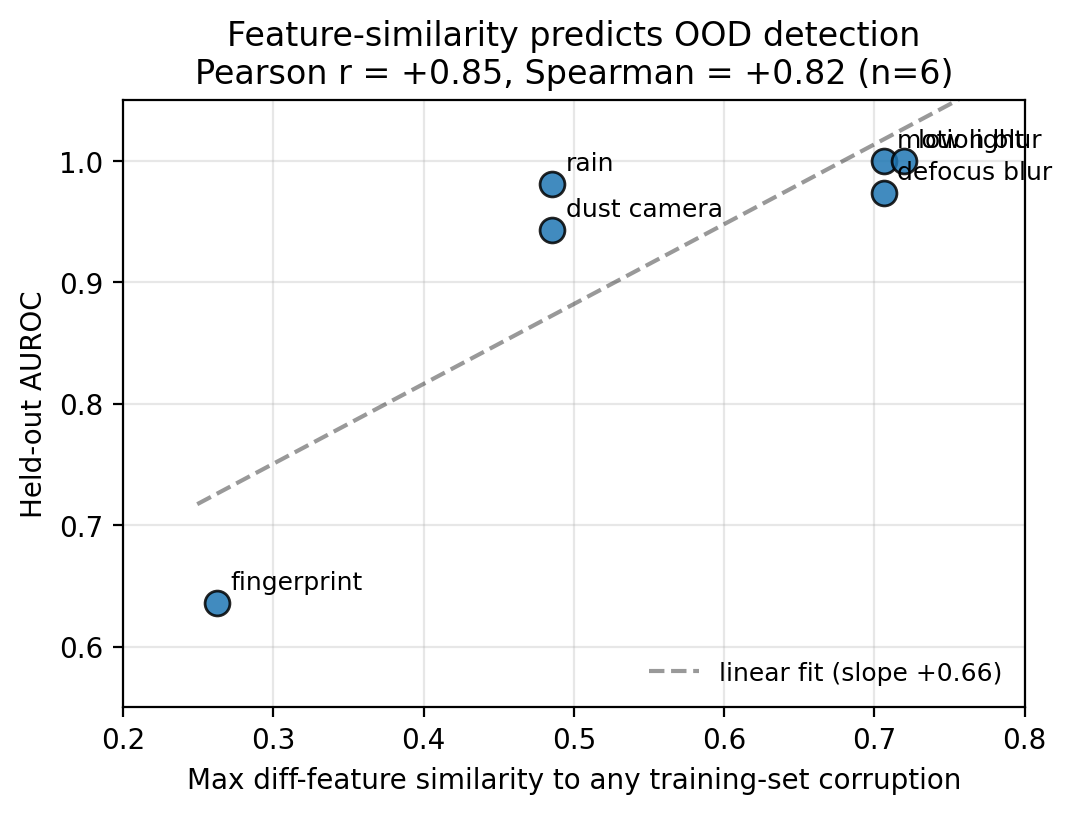
\includegraphics[width=0.92\columnwidth]{figures/ood_predictability.png}
    \caption{Held-out AUROC vs.\ maximum feature-delta cosine similarity to any training-set corruption type. Each point is one LOO fold (the six corruption types that produced measurable failures). Pearson $r = +0.85$, Spearman $\rho_s = +0.82$ ($n=6$): \emph{the more similar a novel corruption's feature-delta is to a training-set corruption, the better the monitor detects its failures}. Naively-similar raw-feature similarity (without the clean-image baseline) shows no such relationship --- the predictive signal is the perturbation direction, not the perturbed point.}
    \label{fig:ood_pred}
\end{figure}

\cref{fig:ood_pred} shows a strong relationship between this similarity and the held-out AUROC across the six failing corruption types: Pearson $r = +0.85$, Spearman $\rho_s = +0.82$.
The two best-detected pairs are exactly the ones we'd predict from physical mechanism: motion blur and defocus blur (both high-frequency suppressors, max delta-sim $= 0.71$, AUROC $\geq 0.97$) and gaussian noise / low-light (both noise-like, max delta-sim $= 0.72$).
Fingerprint, with its idiosyncratic localized whorl-ridge perturbation that no other training corruption matches (max delta-sim $= 0.26$), is correspondingly the hardest to detect (AUROC $= 0.64$).

Two implications:
(i)~\emph{Operationally}: a deployment can predict whether a novel corruption will be reliably detected by computing this cheap delta-similarity statistic on a small sample of clean/corrupted frames, without needing ground-truth failure labels.
(ii)~\emph{Methodologically}: the same delta-similarity matrix could be used at training-set design time to choose corruption types that maximally cover the feature-delta space, increasing the radius of corruption types the monitor can confidently generalize to.
We note the small $n$ (6 valid folds) and recommend reproducing this analysis with a wider corruption taxonomy before drawing strong conclusions about the slope; the qualitative finding --- that delta-direction similarity matters and raw-feature similarity does not (\cref{tab:sim_correlations}) --- is robust to that caveat.

\begin{table}[t]
\centering
\caption{Correlations between feature-similarity statistics (over 6 LOO folds) and held-out OOD performance. Only delta-direction similarity is predictive; raw-feature similarity is not, and is even spuriously \emph{negatively} correlated with $\rho$.}
\label{tab:sim_correlations}
\footnotesize
\setlength{\tabcolsep}{4pt}
\begin{tabular}{@{}lcc@{}}
\toprule
\textbf{Similarity statistic} & \textbf{vs.\ $\rho$} & \textbf{vs.\ AUROC} \\
\midrule
Max raw-feature sim    & $-0.78$ / $-0.93$ & $-0.27$ / $-0.06$ \\
Max delta-feature sim  & $+0.10$ / $+0.07$ & $\mathbf{+0.85}$ / $\mathbf{+0.82}$ \\
Mean delta-feature sim & $+0.31$ / $+0.23$ & $\mathbf{+0.90}$ / $+0.52$ \\
\bottomrule
\multicolumn{3}{l}{\footnotesize Pearson $r$ / Spearman $\rho_s$} \\
\end{tabular}
\end{table}

\subsection{Practical Deployment Considerations}

The safety monitor runs inference on a single frame at p50 latency $\approx 67$\,ms on a CPU baseline (single-thread on an Apple M-series core) and well under 10\,ms on a consumer GPU, making it suitable for real-time deployment alongside the manipulation policy at typical 10--30\,Hz control rates.
The envelope analysis provides deployment-time guidance: operators can specify acceptable risk thresholds and the system reports the maximum occlusion coverage that remains within the certified safe zone.

\subsection{Limitations}

\begin{itemize}
    \item \textbf{Simulation only.} All experiments are conducted in simulation. Real-world camera occlusions may differ in appearance and statistics. A real-world pilot is left for future work.
    \item \textbf{Task scope.} We evaluate on pick-and-place tasks; generalization to contact-rich or long-horizon tasks is untested.
    \item \textbf{Occlusion diversity.} Nine corruption types span the principal physical mechanisms we identified, but real-world deployment will encounter combinations and modes not represented here; the cross-corruption generalization result (\cref{sec:loo}) is the paper's hedge against this gap, but it is not a guarantee.
    \item \textbf{Calibration.} As reported in \cref{sec:calibration}, the monitor is well-ranked (mean $\rho = 0.79$) but only modestly calibrated (pooled ECE $= 0.243$). Probability outputs should be recalibrated for any deployment that consumes them as numeric thresholds rather than as ordering signals.
    \item \textbf{Single policy.} All envelope and LOO results use a single VLA policy (InternVLA-M1). Whether the cross-corruption transfer property holds for other VLA architectures (Octo, RT-2, OpenVLA) is an open question.
\end{itemize}

\subsection{Connection to SOTIF}
\label{sec:sotif}

ISO~21448~\cite{iso21448} partitions the operating scenario space into four quadrants defined by whether a scenario is \emph{known} to the developer and whether it is \emph{safe} under the system under test.
Our two contributions map onto this partition as follows.

\noindent\textbf{Adversarial envelope $\to$ known/unknown unsafe reduction.}
For each corruption type in our taxonomy, the CMA-ES envelope analysis searches parameter space for worst-case configurations at each budget level.
Conditions that yield $\text{SR}^*(\mathcal{O}, \beta) < \tau_{\text{safe}}$ become \emph{known unsafe} --- they are documented, reproducible scenarios at which the policy is certified to fail.
Conditions with $\text{SR}^*(\mathcal{O}, \beta) \geq \tau_{\text{safe}}$ become \emph{known safe} up to the adversarial coverage of our search.
Random testing alone cannot discharge this obligation, because the gap between adversarial and random success rates (\cref{tab:envelope}) shows that typical-case performance systematically overstates worst-case safety.

\noindent\textbf{Cross-corruption monitor $\to$ unknown unsafe coverage.}
The residual SOTIF risk is the \emph{unknown unsafe} quadrant --- corruption modes that were not enumerated during development but occur in deployment (novel lens contaminants, unanticipated weather artifacts, sensor aging patterns).
A monitor that only detects failures under trained corruptions reduces to a lookup table and contributes nothing to this quadrant.
Our LOO evaluation explicitly measures the monitor's ability to detect failures under corruption types \emph{held out from training}, providing evidence that the monitor generalizes to unseen degradation mechanisms and thus transfers risk from the ``unknown unsafe'' quadrant toward ``known unsafe'' at runtime.
The six-corruption mean Spearman $\rho = 0.79$ and AUROC $= 0.92$ quantify this coverage.

\noindent\textbf{Residual limitations.}
Two SOTIF-relevant gaps remain.
First, our envelope analysis presently covers fingerprint and glare only; certifying the full nine-corruption envelope would close known/unknown unsafe for the rest of the taxonomy.
Second, the monitor's coverage of truly novel degradation modes (e.g., sensor-specific hardware faults, physically unmodeled atmospheric optics) can only be estimated; it is the nature of the unknown-unsafe quadrant that its coverage cannot be proved exhaustively, and any SOTIF argument using this monitor must state residual risk accordingly.

% ============================================================================
\section{Conclusion}
\label{sec:conclusion}

We presented a framework for safety monitoring of vision-based manipulation under camera occlusion, combining adversarial envelope analysis with a lightweight cross-corruption safety predictor.
Across nine corruption types spanning six physical mechanisms, the monitor achieves mean Spearman $\rho = 0.79 \pm 0.12$ and mean AUROC $= 0.92 \pm 0.13$ on held-out corruption types not seen during training (restricted to the six types that produce measurable policy failures at the evaluated budgets).
The central finding is that frozen ImageNet features enable a 33K-parameter CNN head to predict failure under occlusion types never encountered during training, suggesting that practical safety monitors need not enumerate every possible degradation mode.
Adversarial CMA-ES search provides certified worst-case bounds, while the cross-corruption monitor provides real-time per-frame risk assessment.
Together, these components address both the ``known unsafe'' and ``unknown unsafe'' quadrants of the SOTIF framework for vision-based manipulation.

% ============================================================================
\section*{Acknowledgments}
This work was conducted as an independent research project.
The author thanks the developers of SimplerEnv, ManiSkill2, and InternVLA-M1 for releasing their tools, and the open-source CMA-ES community.

% ============================================================================
\bibliographystyle{IEEEtran}
\bibliography{references}

\end{document}
